%% Slides for speech about Erlang parse_transofm at Erlang Dnipro 2014
%% https://github.com/Mendor/slides/tree/master/2014-02_erlangdnipro_parse_trans

\documentclass[10pt]{beamer}

\usepackage{PTSans}
\usepackage{PTMono}
\usepackage[T1]{fontenc}
\usepackage[utf8]{inputenc}
\usepackage[english,russian]{babel}
\usepackage{verbatim}
\usepackage{alltt}
\usepackage{graphicx}
\usepackage{multicol}
\usepackage[absolute,overlay]{textpos}

% Beamer theme
\usetheme{Antibes}
\usecolortheme{beaver}
% \setbeamerfont{title}[default][size=Huge]
\setbeamertemplate{frametitle}[default][center]
\setbeamertemplate{blocks}[rounded][shadow=true]
\setbeamercolor{frametitle}{bg=white!10!white}

\newcommand\RightBottom[1]{%
    \begin{textblock*}{\paperwidth}(8.5cm,7.5cm)
        \raggedright #1\hspace{.5em}
    \end{textblock*}}

% Presentation meta
\title[Erlang Dnipro 2014]{parse\_transform и все-все-все}
\date{15 февраля, 2014}
\author{Никита Калашников}

\begin{document}

    % 01
    \frame{\titlepage}

    % 02
    \begin{frame}[c]
        \frametitle{}
        \LARGE\begin{center}
            {\color{darkred} Нелирическое вступление №1:\\процесс компиляции}
        \end{center}
    \end{frame}

    % 03
    \begin{frame}
        \frametitle{Процесс компиляции\\{\normalsize (не только в Erlang и в общих чертах)}}
        \begin{enumerate}
            \item Исходный код.
            \item Обработанный код.
            \item Синтаксическое дерево.
            \item Байт-код.
        \end{enumerate}
    \end{frame}

    % 04
    \begin{frame}
        \frametitle{Процесс компиляции\\{\normalsize (не только в Erlang и в общих чертах)}}
        \begin{enumerate}
            \item Исходный код.
            \item Обработанный код.
            \item \textbf{Синтаксическое дерево.}
            \item Байт-код.
        \end{enumerate}
    \end{frame}

    % 05
    \begin{frame}
        \frametitle{Синтаксическое дерево\\{\normalsize Оно же дерево разбора, дерево вывода}}
        Результат группировки токенов исходного кода программы в грамматические фразы синтаксическим
        анализатором. \vspace{0.5cm} \\

        Абстрактное синтаксическое дерево — подвид дерева разбора, отличающийся тем, что в нём отсутствуют
        элементы для токенов, которые не влияют на семантику программы.
        \begin{center}
            \texttt{x3 := y + 3; } \hspace{1cm}
            \raisebox{-1.3cm}{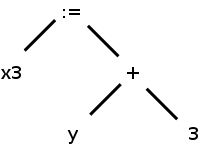
\includegraphics[width=100pt]{assets/syntaxtree.png}}
        \end{center}
    \end{frame}

    % 06
    \begin{frame}[c]
        \frametitle{}
        \LARGE\begin{center}
            {\color{darkred} Нелирическое вступление №2:\\самый известный пример деревьев}
        \end{center}
    \end{frame}

    % 07
    \begin{frame}
        \frametitle{Lisp и его синтаксис}
        \begin{block}{}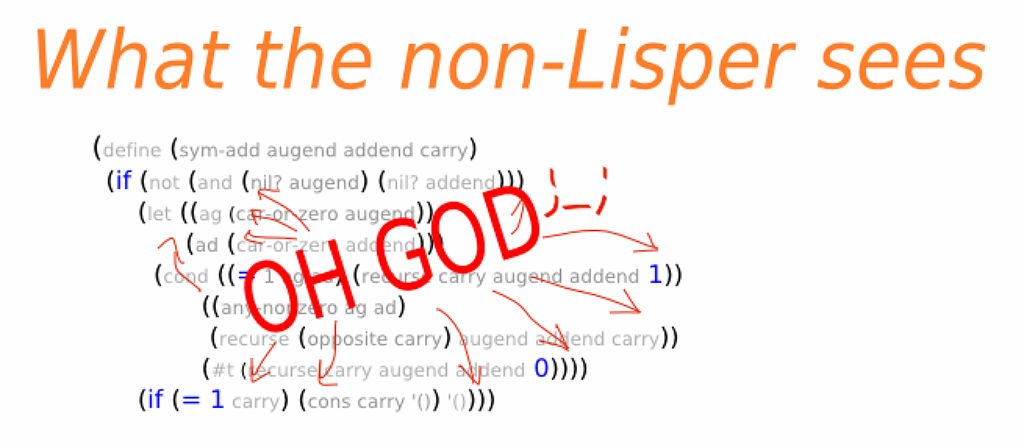
\includegraphics[width=\textwidth]{assets/lispomg.jpg}\end{block}
    \end{frame}

    % 08
    \begin{frame}
        \frametitle{Lisp и его синтаксис}
        \begin{multicols}{2}
            На самом деле синтаксиса нет. Код на Lisp сам по себе является синтаксическим деревом.
            {\scriptsize \verbatiminput{assets/sample.lisp}}
            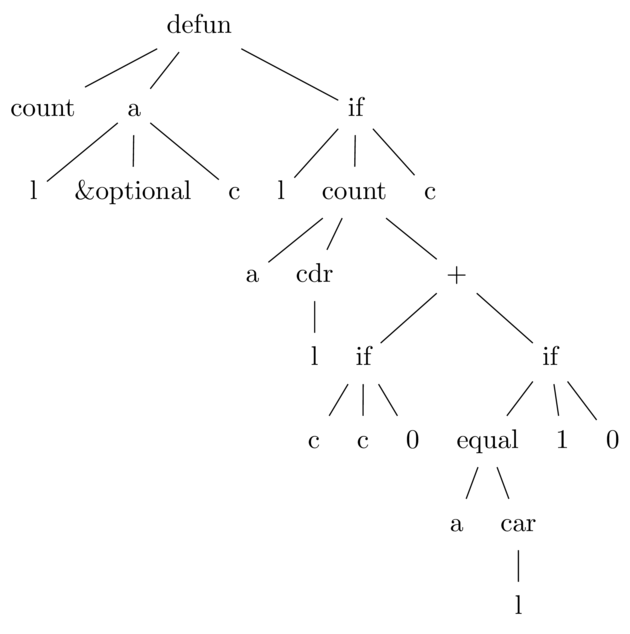
\includegraphics[width=150pt]{assets/lisptree.png}
        \end{multicols}
    \end{frame}

    % 09
    \begin{frame}[c]
        \frametitle{}
        \huge\begin{center}
            {\color{darkred}К чему всё это?}
        \end{center}
    \end{frame}

    % 10
    \begin{frame}
        \frametitle{Erlang Abstract Format}
        Местные синтаксические деревья. Представление исходного кода программы в термах Erlang. \vspace{0.2cm} \\
        \begin{center}
        {\small \verbatiminput{assets/factorial.erl}}
        \begin{picture}(1,1)
            \vector(0,-1){15}
        \end{picture}
        \vspace{0.5cm} \\
        \begin{alltt}
epp:parse\_file(''factorial.erl'', [], []).
        \end{alltt}
        \end{center}
        % epp:parse_file("factorial.erl", [], []).
        % \begin{verbatim}
        %     ololo
        % \end{verbatim}
    \end{frame}

    % 11
    \begin{frame}
        \frametitle{Erlang Abstract Format}
        {\scriptsize \verbatiminput{assets/factorial.forms}}
    \end{frame}

    % 12
    \begin{frame}
        \frametitle{parse\_transform}
        Изменение дерева Erlang Abstract Format в процессе компиляции в пределах возможностей синтаксиса языка
        с помощью другого Erlang-кода. То есть метапрограммирование.
    \end{frame}

    % 13
    \begin{frame}
        \frametitle{parse\_transform\\{\normalsize Глазами разрабочика}}
        Файл трансформаций — обычный модуль Erlang с единственной экспортируемой функцией \texttt{parse\_transform/2},
        которая принимает на вход абстрактное дерево оригинального исходного кода и возвращает изменённое.\vspace{1cm} \\

        Модуль, который нужно трансформировать, компилируется с опцией \texttt{\{parse\_transform, your\_transform\_module\}}.
    \end{frame}

    % 14
    \begin{frame}[c]
        \frametitle{}
        \huge\begin{center}
            {\color{darkred}Примеры из жизни?}
        \end{center}
    \end{frame}

    % 15
    \begin{frame}[t]
        \frametitle{lager}
        \begin{center}
            \underline{\href{https://github.com/basho/lager}{github.com/basho/lager}}
        \end{center}
        
        Фреймворк для логгирования. Использует parse\_transform для преобразования вызовов вроде \texttt{lager:info()}
        в структуру, также включающую в себя метаданные вызова (например, дату, имя модуля, номер строки и т. д.)\vspace{0.5cm} \\

        \begin{alltt}
lager:info(''Logged in as {\textasciitilde}s'', [Username]),
        \end{alltt}
        \begin{center}
        \begin{picture}(1,1)
            \vector(0,-1){15}
        \end{picture}
        \end{center}\vspace{0.5cm}
        \footnotesize\begin{alltt}
2014-01-11 13:12:44.109 [info] <0.118.0>@app\_core:login:203 Logged in as someuser
        \end{alltt}
        
    \end{frame}

    % 16
    \begin{frame}[t]
        \frametitle{erlando}
        \begin{center}
            \underline{\href{https://github.com/rabbitmq/erlando}{github.com/rabbitmq/erlando}}
        \end{center}
        
        Набор синтаксических расширений (карринг, do-нотация, импорт функций из других модулей).\vspace{0.3cm} \\

        Например, использование реализации монады Error:\\
        {\scriptsize \verbatiminput{assets/error.erl}}

        вместо дерева проверяющих \texttt{case}'ов на каждый вызов.
    \end{frame}

    % 17
    \begin{frame}[t]
        \frametitle{shen}
        \begin{center}
            \underline{\href{https://github.com/5HT/shen}{github.com/5HT/shen}}
        \end{center}
        
        Трансляция Erlang в JavaScript :). Полностью строит JS-код из Erlang Abstract Format.\vspace{0.5cm} \\

        \begin{multicols}{2}
            {\tiny \verbatiminput{assets/fac.erl}}
            {\tiny \verbatiminput{assets/fac.js}}
        \end{multicols}
    \end{frame}

    % 18
    \begin{frame}
        \frametitle{Бочка дёгтя\\{\normalsize при использовании parse\_transform}}
        \begin{itemize}
            \item Из-за появления неявных преобразований код становится менее очевиден.
            \item Дополнительные сложности в отладке (необходимость учитывать трансформации, потеря
                возможности диалайзинга исходного кода до трансформаций).
            \item Придумать свой диалект Erlang всё равно не получится.
        \end{itemize} \vspace{1cm}

        \textbf{Писать собственные трансформации стоит с предельной осторожностью! Чуть реже, чем всегда,
            можно обойтись без подобных глубинных вмешательств.}
    \end{frame}

    % 19
    \begin{frame}[c]
        \frametitle{}
        \huge\begin{center}
            {\color{darkred} Спасибо!\\Вопросы?}
        \end{center}

        \RightBottom{\normalsizeНикита Калашников \vspace{1mm} \\
        \footnotesize\raisebox{-1mm}{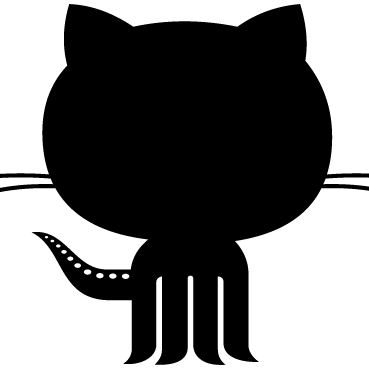
\includegraphics[width=0.3cm]{assets/github.png}}
            \underline{\href{https://github.com/Mendor}{github.com/Mendor}} \vspace{1mm} \\
        \raisebox{-1mm}{
\includegraphics[width=0.3cm]{assets/twitter.png}}
            \underline{\href{https://twitter.com/archydragon}{twitter.com/archydragon}}\\}
    \end{frame}

    % 99
    \begin{frame}
        \footnotesize\textit{This slide is intentionally left blank.}
    \end{frame}

\end{document}
